\documentclass[a4paper,12pt]{article}

\usepackage{hyperref}
\usepackage{amsmath}
\usepackage{enumitem}
\usepackage{graphicx}
\usepackage{fancyhdr}

\title{Memory Data Bus Transition Count \\ Progress Report 1}
\date{\today}
%\author{John Doe\\ Magic Department\thanks{I am no longer a member of this department}, Richard Miles University 

\begin{document}
%\maketitle
\fancyhf{}
\pagestyle{fancy}
\cfoot{\thepage}
\renewcommand{\headrulewidth}{0pt}
\renewcommand{\footrulewidth}{0.4pt}


\section{Objective}
Create a tool which will count the number of bit transitions on the memory data bus, which can instrument realistic programs.

\section{Short Introduction}
We have used Intel Pin to implement the tool as discussed.

Intel Pin provides a very simple mechanism to instrument all memory accesses of the program it attaches to, so it is straightforward to detect every read/write operation.

The problem here was, \textbf{there is no way to detect which memory accesses are actually done to the external memory using Intel Pin}, as it can only detect the calls the program makes. In a realistic scenario with a standard cache implementation, most of the accesses would be to the internal caches, and only in the case of the last level cache miss the memory would have been accessed. Our solution to this was \textbf{to simulate a simple cache hierarchy and count the number of transitions on the data bus only when the unified L3 cache has a miss.} 

\section{Pin Tool Implementation}
We have examined the tools supplied by Intel, and found out that there is a tool named \emph{allcache}\footnote{location: pin/source/tools/memory/allcache.cpp} which simulates the following:
\begin{itemize}
\item Separate L1 caches for data and instruction
\item Unified L2 and L3 caches
\item Separate TLB for data and instruction
\end{itemize}

The cache parameters are easily configured, however \textbf{the tool can only simulate the architecture of a single core cache hierarchy.} We assumed that this tool would be a good enough starting point, so we decided \textbf{to modify the tool slightly to allow us to count the transitions in case of L3 misses.} 

The supplied tool was already able to detect L3 misses, however the accesses were done in bulk and it was reported as a miss in case of any of the accesses being a miss. \textbf{We have replaced the bulk access function with a single line access function (in a loop) to detect the misses at line access granularity. We have also added the necessary code to copy the data (using \emph{PIN\_SafeCopy}) residing in memory to a buffer and then do the actual transition counting.}

\subsection{Transition Counting}
We have assumed that the memory is accessed with the granularity of the L3 cache line size (typically 64B). After doing some research into how DDR SDRAM read/write operations work, we have understood that the typical bus width is 8B (+1B in case of error correction), so the data is read in bursts of up to 8 (or lower and more concatenated read operations) to accomodate for the L3 cache line size.

The data bus is in a high impedance state when no read/write operations are being carried out, so in our implementation we ignored the transition count from the high impedance state to the first word (8B in size) being read/written. We also do not count the transitions from the last word to the high impedance state.

To count the number of transitions on the data bus, we have implemented a \textbf{look up table (LUT)} with size 256*256 (64kB). The row is chosen by the first byte to be compared, and the column is chosen by the second one. The read result is a single byte value between 0 to 8. To fill the look up table the tool calls an initialization function which calculates \textbf{the hamming distance} between the two bytes using a xor to set the differing bytes and then applying Brian Kernighan's algorithm\footnote{https://graphics.stanford.edu/~seander/bithacks.html\#CountBitsSetKernighan} to count the number of bits inside a byte. 

The number of transitions are counted and accumulated for every byte of neighboring 8B words (i.e. bus width) being transmitted as shown in \hyperref[fig_1]{Figure 1}. 

\begin{figure}[h]
		\label{fig_1}
		\centering
		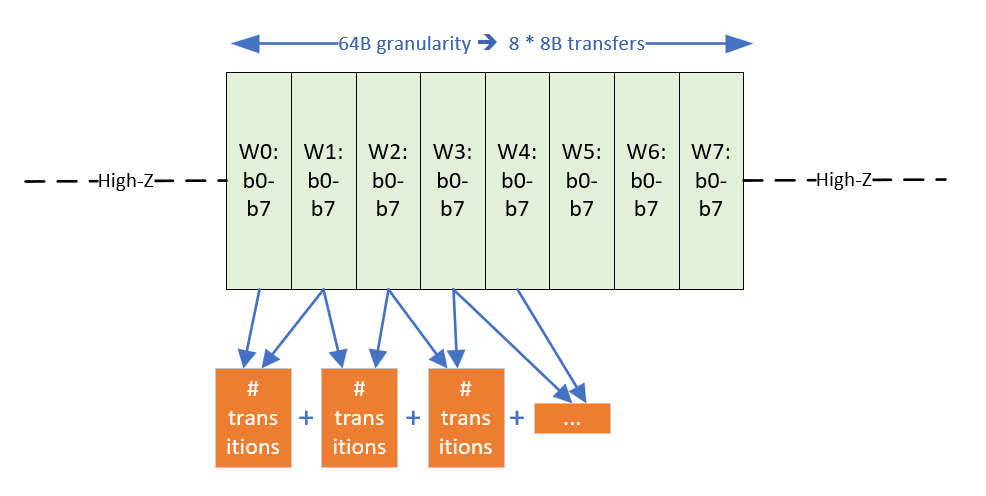
\includegraphics[scale=0.5]{databus_1.png}
		\caption{Calculating the transition count on the memory data bus}
\end{figure}

\section{Output}
The default \emph{allcache} tool outputs the cache and TLB access/hit/miss statistics and miss ratios. As we have built on top of the existing tool, we have kept this output format and added the number of bit transitions to the bottom as shown in \hyperref[fig_2]{Figure 2}.

\begin{figure}[h]
		\label{fig_2}
		\centering
		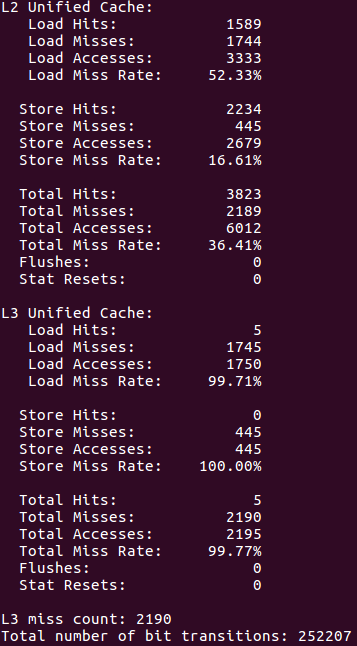
\includegraphics[scale=1]{output_1.png}
		\caption{Tool output for linux ls}
\end{figure}

\end{document}